% Build: tectonic report.tex   (chart.tex is generated by `jacobian_transfers chart --tikz chart.tex`)
\documentclass[10pt]{article}
\usepackage[margin=2cm]{geometry}
\usepackage{amsmath,amssymb}
\usepackage{tikz}
\usepackage{booktabs}
\usepackage{longtable}
\usepackage{hyperref}
\usepackage{xcolor}
\usetikzlibrary{arrows.meta,positioning,shapes.misc}
\title{Jacobian transfer discovery across the curve registry\\ \large automated screen, 2026-10-10}
\author{crypto repository, \texttt{jacobian\_transfers}}
\date{2026-10-10}
\begin{document}
\maketitle

\section*{Question and answer}
For each of the \textbf{321
} curves in \texttt{docs/curves/registry.json}, can its discrete
logarithm be moved into the Jacobian of a curve of higher genus at a cost the literature's
complexity formulas place below Pollard rho on the original subgroup?  The native screen
(\texttt{src/cryptanalysis/jacobian\_transfer/}) enumerates the known routes, computes what
is exact (GHS magic numbers and genera for every field factorisation, same-field cover
genera and degrees, 2-torsion signals, the census of curves with small Frobenius
annihilators), and prices the rest with one frozen formula cost model.  Every row is a
formula.  A \emph{formula advantage} is a lead with open obligations; a \emph{boundary}
is a route the formulas themselves put at or above rho.

\section*{Routes}
\begin{center}
\resizebox{\textwidth}{!}{% TikZ rendering of routes.svg (the SVG is the docs copy; both are hand-maintained from the same list in JACOBIAN_TRANSFERS.md)
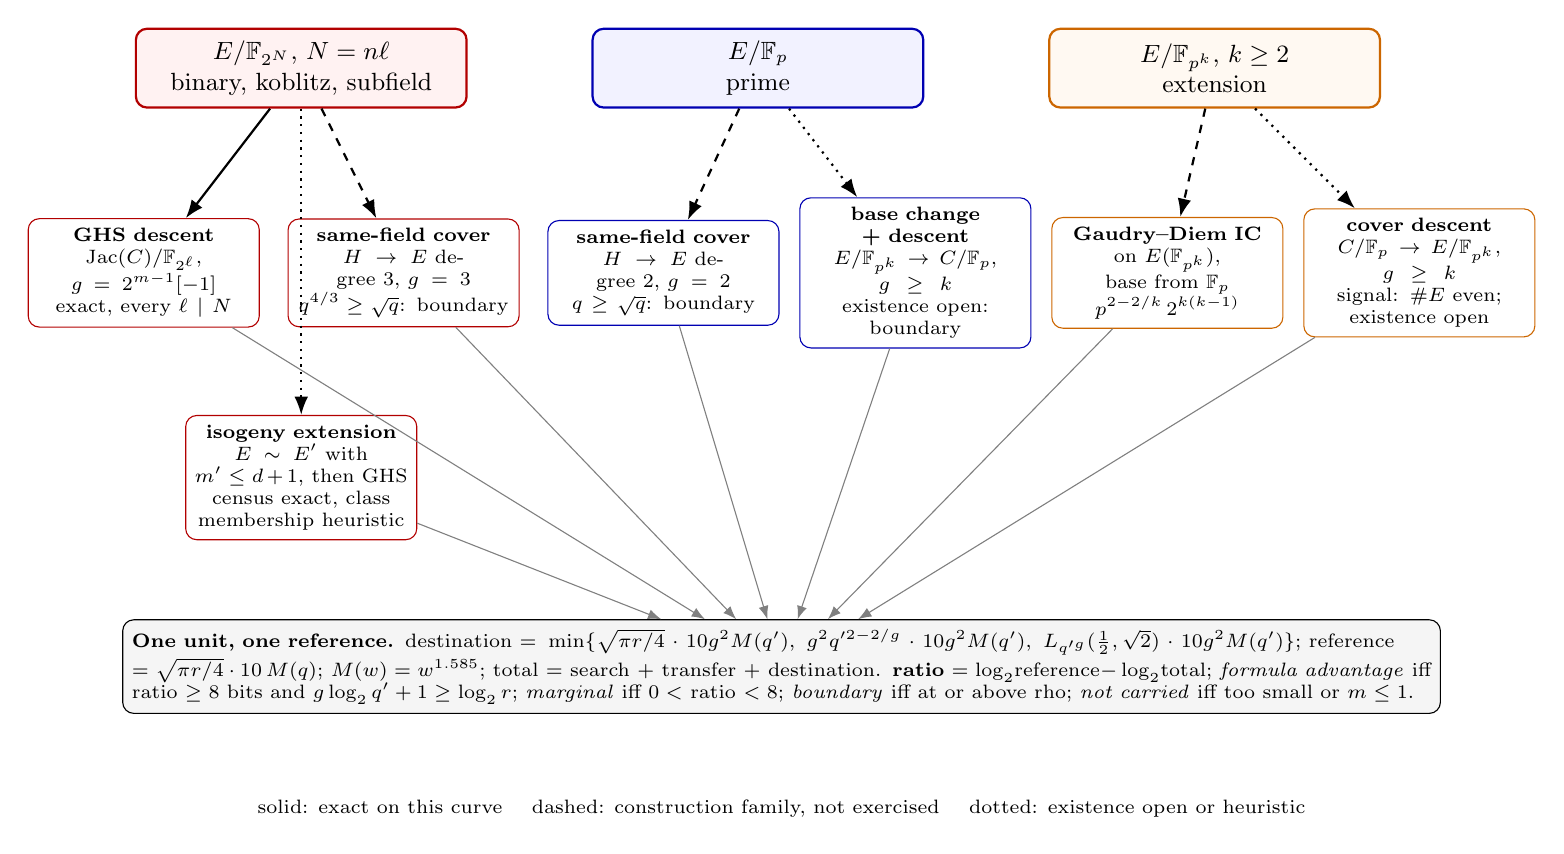
\begin{tikzpicture}[
  src/.style={draw,rounded corners,minimum width=4.2cm,minimum height=1cm,align=center,font=\small,thick},
  dst/.style={draw,rounded corners,minimum width=2.9cm,align=center,font=\scriptsize,text width=2.7cm},
  exact/.style={-{Latex},thick},
  cons/.style={-{Latex},thick,dashed},
  open/.style={-{Latex},thick,dotted},
  x=1cm,y=1cm]
\node[src,draw=red!70!black,fill=red!5] (bin) at (0,0) {$E/\mathbb F_{2^N}$, $N=n\ell$\\ binary, koblitz, subfield};
\node[src,draw=blue!70!black,fill=blue!5] (pri) at (5.8,0) {$E/\mathbb F_p$\\ prime};
\node[src,draw=orange!80!black,fill=orange!5] (ext) at (11.6,0) {$E/\mathbb F_{p^k}$, $k\ge2$\\ extension};
\node[dst,draw=red!70!black] (ghs) at (-2.0,-2.6) {\textbf{GHS descent}\\ $\mathrm{Jac}(C)/\mathbb F_{2^\ell}$, $g=2^{m-1}[-1]$\\ exact, every $\ell\mid N$};
\node[dst,draw=red!70!black] (iso) at (0,-5.2) {\textbf{isogeny extension}\\ $E\sim E'$ with $m'\le d+1$, then GHS\\ census exact, class membership heuristic};
\node[dst,draw=red!70!black] (sfb) at (1.3,-2.6) {\textbf{same-field cover}\\ $H\to E$ degree 3, $g=3$\\ $q^{4/3}\ge\sqrt q$: boundary};
\node[dst,draw=blue!70!black] (sfp) at (4.6,-2.6) {\textbf{same-field cover}\\ $H\to E$ degree 2, $g=2$\\ $q\ge\sqrt q$: boundary};
\node[dst,draw=blue!70!black] (bcd) at (7.8,-2.6) {\textbf{base change + descent}\\ $E/\mathbb F_{p^k}\to C/\mathbb F_p$, $g\ge k$\\ existence open: boundary};
\node[dst,draw=orange!80!black] (gd) at (11.0,-2.6) {\textbf{Gaudry--Diem IC}\\ on $E(\mathbb F_{p^k})$, base from $\mathbb F_p$\\ $p^{2-2/k}\,2^{k(k-1)}$};
\node[dst,draw=orange!80!black] (cd) at (14.2,-2.6) {\textbf{cover descent}\\ $C/\mathbb F_p\to E/\mathbb F_{p^k}$, $g\ge k$\\ signal: $\#E$ even; existence open};
\draw[exact] (bin) -- (ghs);
\draw[open] (bin) -- (iso);
\draw[cons] (bin) -- (sfb);
\draw[cons] (pri) -- (sfp);
\draw[open] (pri) -- (bcd);
\draw[cons] (ext) -- (gd);
\draw[open] (ext) -- (cd);
\node[draw,fill=gray!8,rounded corners,text width=16.5cm,align=left,font=\scriptsize] (price) at (6.1,-7.6) {
\textbf{One unit, one reference.} destination $=\min\{\sqrt{\pi r/4}\cdot10g^2 M(q'),\ g^2q'^{2-2/g}\cdot10g^2M(q'),\ L_{q'^g}(\tfrac12,\sqrt2)\cdot10g^2M(q')\}$;
reference $=\sqrt{\pi r/4}\cdot10\,M(q)$; $M(w)=w^{1.585}$; total $=$ search $+$ transfer $+$ destination.
\textbf{ratio} $=\log_2$reference$-\log_2$total; \emph{formula advantage} iff ratio $\ge8$ bits and $g\log_2q'+1\ge\log_2 r$; \emph{marginal} iff $0<$ ratio $<8$; \emph{boundary} iff at or above rho; \emph{not carried} iff too small or $m\le1$.};
\draw[-{Latex},gray] (ghs) -- (price); \draw[-{Latex},gray] (iso) -- (price); \draw[-{Latex},gray] (sfb) -- (price);
\draw[-{Latex},gray] (sfp) -- (price); \draw[-{Latex},gray] (bcd) -- (price); \draw[-{Latex},gray] (gd) -- (price); \draw[-{Latex},gray] (cd) -- (price);
\node[font=\scriptsize,align=center] at (6.1,-9.4) {solid: exact on this curve \quad dashed: construction family, not exercised \quad dotted: existence open or heuristic};
\end{tikzpicture}
}
\end{center}

\section*{Ratio of the best carried route to rho, every curve}
\begin{center}
\resizebox{\textwidth}{!}{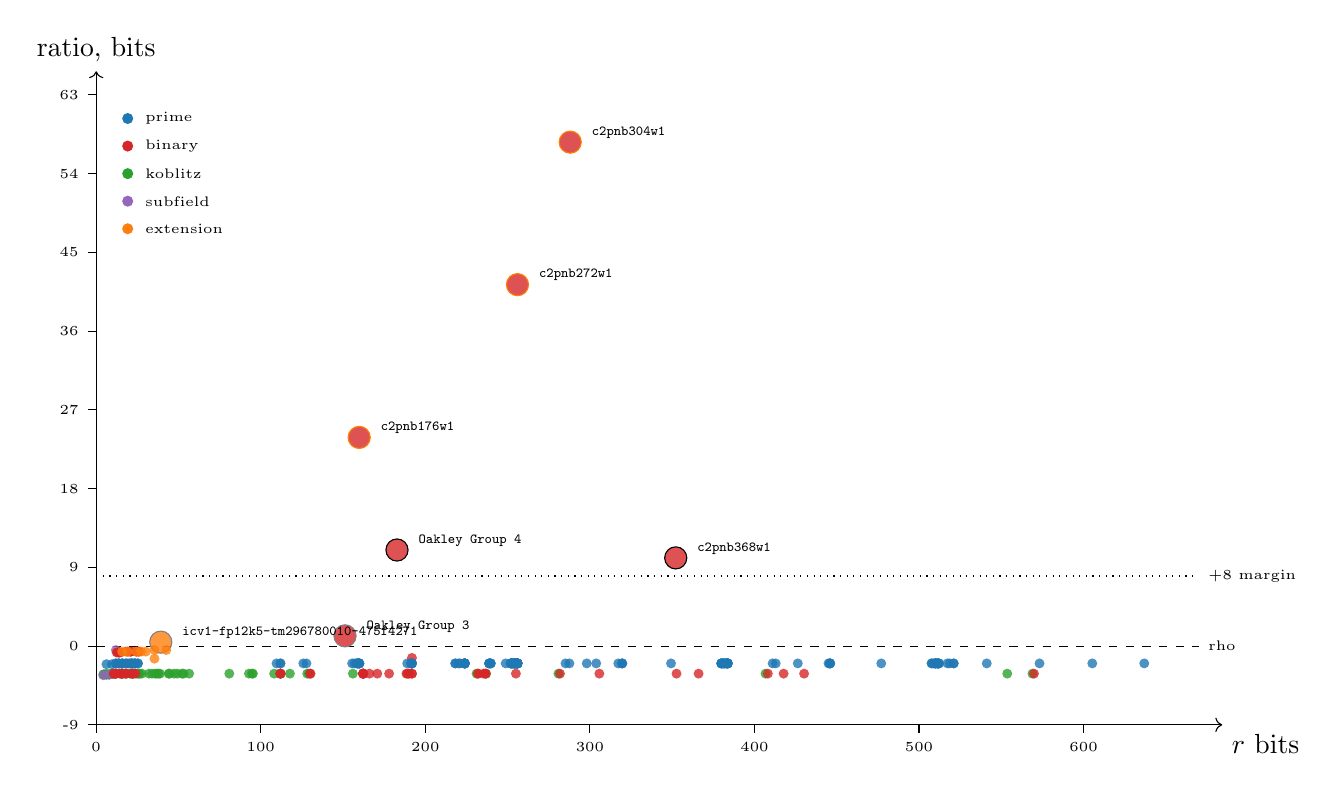
\begin{tikzpicture}[x=1cm,y=1cm]
\draw[->] (0,0) -- (14.30,0) node[below right] {$r$ bits};
\draw[->] (0,0) -- (0,8.30) node[above] {ratio, bits};
\draw (0.00,0) -- ++(0,-0.1) node[below] {\tiny 0};
\draw (2.09,0) -- ++(0,-0.1) node[below] {\tiny 100};
\draw (4.18,0) -- ++(0,-0.1) node[below] {\tiny 200};
\draw (6.27,0) -- ++(0,-0.1) node[below] {\tiny 300};
\draw (8.36,0) -- ++(0,-0.1) node[below] {\tiny 400};
\draw (10.45,0) -- ++(0,-0.1) node[below] {\tiny 500};
\draw (12.54,0) -- ++(0,-0.1) node[below] {\tiny 600};
\draw (0,0.00) -- ++(-0.1,0) node[left] {\tiny -9};
\draw (0,1.00) -- ++(-0.1,0) node[left] {\tiny 0};
\draw (0,2.00) -- ++(-0.1,0) node[left] {\tiny 9};
\draw (0,3.00) -- ++(-0.1,0) node[left] {\tiny 18};
\draw (0,4.00) -- ++(-0.1,0) node[left] {\tiny 27};
\draw (0,5.00) -- ++(-0.1,0) node[left] {\tiny 36};
\draw (0,6.00) -- ++(-0.1,0) node[left] {\tiny 45};
\draw (0,7.00) -- ++(-0.1,0) node[left] {\tiny 54};
\draw (0,8.00) -- ++(-0.1,0) node[left] {\tiny 63};
\draw[dashed] (0,1.00) -- (14.00,1.00) node[right] {\tiny rho};
\draw[dotted] (0,1.89) -- (14.00,1.89) node[right] {\tiny +8 margin};
\fill[fill={rgb,255:red,44;green,160;blue,44},fill opacity=0.8] (0.10,0.64) circle (1.8pt);
\fill[fill={rgb,255:red,44;green,160;blue,44},fill opacity=0.8] (0.13,0.64) circle (1.8pt);
\fill[fill={rgb,255:red,44;green,160;blue,44},fill opacity=0.8] (0.15,0.64) circle (1.8pt);
\fill[fill={rgb,255:red,44;green,160;blue,44},fill opacity=0.8] (0.11,0.64) circle (1.8pt);
\fill[fill={rgb,255:red,44;green,160;blue,44},fill opacity=0.8] (0.09,0.64) circle (1.8pt);
\fill[fill={rgb,255:red,44;green,160;blue,44},fill opacity=0.8] (0.21,0.65) circle (1.8pt);
\fill[fill={rgb,255:red,44;green,160;blue,44},fill opacity=0.8] (0.21,0.65) circle (1.8pt);
\fill[fill={rgb,255:red,44;green,160;blue,44},fill opacity=0.8] (0.23,0.65) circle (1.8pt);
\fill[fill={rgb,255:red,44;green,160;blue,44},fill opacity=0.8] (0.13,0.64) circle (1.8pt);
\fill[fill={rgb,255:red,44;green,160;blue,44},fill opacity=0.8] (0.13,0.64) circle (1.8pt);
\fill[fill={rgb,255:red,44;green,160;blue,44},fill opacity=0.8] (0.20,0.65) circle (1.8pt);
\fill[fill={rgb,255:red,44;green,160;blue,44},fill opacity=0.8] (0.16,0.64) circle (1.8pt);
\fill[fill={rgb,255:red,44;green,160;blue,44},fill opacity=0.8] (0.16,0.64) circle (1.8pt);
\fill[fill={rgb,255:red,44;green,160;blue,44},fill opacity=0.8] (0.17,0.64) circle (1.8pt);
\fill[fill={rgb,255:red,44;green,160;blue,44},fill opacity=0.8] (0.33,0.65) circle (1.8pt);
\fill[fill={rgb,255:red,44;green,160;blue,44},fill opacity=0.8] (0.36,0.65) circle (1.8pt);
\fill[fill={rgb,255:red,44;green,160;blue,44},fill opacity=0.8] (0.38,0.65) circle (1.8pt);
\fill[fill={rgb,255:red,44;green,160;blue,44},fill opacity=0.8] (0.13,0.64) circle (1.8pt);
\fill[fill={rgb,255:red,44;green,160;blue,44},fill opacity=0.8] (0.44,0.65) circle (1.8pt);
\fill[fill={rgb,255:red,44;green,160;blue,44},fill opacity=0.8] (0.46,0.65) circle (1.8pt);
\fill[fill={rgb,255:red,44;green,160;blue,44},fill opacity=0.8] (0.46,0.65) circle (1.8pt);
\fill[fill={rgb,255:red,44;green,160;blue,44},fill opacity=0.8] (0.32,0.65) circle (1.8pt);
\fill[fill={rgb,255:red,44;green,160;blue,44},fill opacity=0.8] (0.32,0.65) circle (1.8pt);
\fill[fill={rgb,255:red,44;green,160;blue,44},fill opacity=0.8] (0.43,0.65) circle (1.8pt);
\fill[fill={rgb,255:red,44;green,160;blue,44},fill opacity=0.8] (0.32,0.65) circle (1.8pt);
\fill[fill={rgb,255:red,44;green,160;blue,44},fill opacity=0.8] (0.32,0.65) circle (1.8pt);
\fill[fill={rgb,255:red,44;green,160;blue,44},fill opacity=0.8] (0.58,0.65) circle (1.8pt);
\fill[fill={rgb,255:red,44;green,160;blue,44},fill opacity=0.8] (0.54,0.65) circle (1.8pt);
\fill[fill={rgb,255:red,44;green,160;blue,44},fill opacity=0.8] (0.81,0.65) circle (1.8pt);
\fill[fill={rgb,255:red,44;green,160;blue,44},fill opacity=0.8] (0.67,0.65) circle (1.8pt);
\fill[fill={rgb,255:red,44;green,160;blue,44},fill opacity=0.8] (0.52,0.65) circle (1.8pt);
\fill[fill={rgb,255:red,44;green,160;blue,44},fill opacity=0.8] (0.77,0.65) circle (1.8pt);
\fill[fill={rgb,255:red,44;green,160;blue,44},fill opacity=0.8] (0.92,0.65) circle (1.8pt);
\fill[fill={rgb,255:red,44;green,160;blue,44},fill opacity=0.8] (0.79,0.65) circle (1.8pt);
\fill[fill={rgb,255:red,44;green,160;blue,44},fill opacity=0.8] (0.93,0.65) circle (1.8pt);
\fill[fill={rgb,255:red,44;green,160;blue,44},fill opacity=0.8] (0.99,0.65) circle (1.8pt);
\fill[fill={rgb,255:red,44;green,160;blue,44},fill opacity=0.8] (0.55,0.65) circle (1.8pt);
\fill[fill={rgb,255:red,44;green,160;blue,44},fill opacity=0.8] (0.75,0.65) circle (1.8pt);
\fill[fill={rgb,255:red,44;green,160;blue,44},fill opacity=0.8] (1.09,0.65) circle (1.8pt);
\fill[fill={rgb,255:red,44;green,160;blue,44},fill opacity=0.8] (1.03,0.65) circle (1.8pt);
\fill[fill={rgb,255:red,44;green,160;blue,44},fill opacity=0.8] (1.18,0.65) circle (1.8pt);
\fill[fill={rgb,255:red,44;green,160;blue,44},fill opacity=0.8] (0.71,0.65) circle (1.8pt);
\fill[fill={rgb,255:red,44;green,160;blue,44},fill opacity=0.8] (1.69,0.65) circle (1.8pt);
\fill[fill={rgb,255:red,44;green,160;blue,44},fill opacity=0.8] (1.11,0.65) circle (1.8pt);
\fill[fill={rgb,255:red,44;green,160;blue,44},fill opacity=0.8] (1.99,0.65) circle (1.8pt);
\fill[fill={rgb,255:red,44;green,160;blue,44},fill opacity=0.8] (1.98,0.65) circle (1.8pt);
\fill[fill={rgb,255:red,44;green,160;blue,44},fill opacity=0.8] (2.70,0.65) circle (1.8pt);
\fill[fill={rgb,255:red,44;green,160;blue,44},fill opacity=0.8] (2.26,0.65) circle (1.8pt);
\fill[fill={rgb,255:red,44;green,160;blue,44},fill opacity=0.8] (1.94,0.65) circle (1.8pt);
\fill[fill={rgb,255:red,44;green,160;blue,44},fill opacity=0.8] (3.26,0.65) circle (1.8pt);
\fill[fill={rgb,255:red,44;green,160;blue,44},fill opacity=0.8] (3.39,0.65) circle (1.8pt);
\fill[fill={rgb,255:red,44;green,160;blue,44},fill opacity=0.8] (2.46,0.65) circle (1.8pt);
\fill[fill={rgb,255:red,44;green,160;blue,44},fill opacity=0.8] (2.68,0.65) circle (1.8pt);
\fill[fill={rgb,255:red,44;green,160;blue,44},fill opacity=0.8] (4.83,0.65) circle (1.8pt);
\fill[fill={rgb,255:red,44;green,160;blue,44},fill opacity=0.8] (4.95,0.65) circle (1.8pt);
\fill[fill={rgb,255:red,44;green,160;blue,44},fill opacity=0.8] (5.87,0.65) circle (1.8pt);
\fill[fill={rgb,255:red,44;green,160;blue,44},fill opacity=0.8] (8.50,0.65) circle (1.8pt);
\fill[fill={rgb,255:red,44;green,160;blue,44},fill opacity=0.8] (11.89,0.65) circle (1.8pt);
\fill[fill={rgb,255:red,44;green,160;blue,44},fill opacity=0.8] (11.57,0.65) circle (1.8pt);
\fill[fill={rgb,255:red,148;green,103;blue,189},fill opacity=0.8] (0.09,0.63) circle (1.8pt);
\fill[fill={rgb,255:red,148;green,103;blue,189},fill opacity=0.8] (0.17,0.64) circle (1.8pt);
\fill[fill={rgb,255:red,148;green,103;blue,189},fill opacity=0.8] (0.25,0.65) circle (1.8pt);
\fill[fill={rgb,255:red,148;green,103;blue,189},fill opacity=0.8] (0.25,0.95) circle (1.8pt);
\fill[fill={rgb,255:red,214;green,39;blue,40},fill opacity=0.8] (0.25,0.65) circle (1.8pt);
\fill[fill={rgb,255:red,214;green,39;blue,40},fill opacity=0.8] (0.25,0.65) circle (1.8pt);
\fill[fill={rgb,255:red,214;green,39;blue,40},fill opacity=0.8] (0.25,0.65) circle (1.8pt);
\fill[fill={rgb,255:red,214;green,39;blue,40},fill opacity=0.8] (0.23,0.65) circle (1.8pt);
\fill[fill={rgb,255:red,214;green,39;blue,40},fill opacity=0.8] (0.22,0.65) circle (1.8pt);
\fill[fill={rgb,255:red,214;green,39;blue,40},fill opacity=0.8] (0.29,0.92) circle (1.8pt);
\fill[fill={rgb,255:red,214;green,39;blue,40},fill opacity=0.8] (0.27,0.92) circle (1.8pt);
\fill[fill={rgb,255:red,214;green,39;blue,40},fill opacity=0.8] (0.29,0.92) circle (1.8pt);
\fill[fill={rgb,255:red,214;green,39;blue,40},fill opacity=0.8] (0.29,0.92) circle (1.8pt);
\fill[fill={rgb,255:red,214;green,39;blue,40},fill opacity=0.8] (0.26,0.92) circle (1.8pt);
\fill[fill={rgb,255:red,214;green,39;blue,40},fill opacity=0.8] (0.29,0.92) circle (1.8pt);
\fill[fill={rgb,255:red,214;green,39;blue,40},fill opacity=0.8] (0.33,0.65) circle (1.8pt);
\fill[fill={rgb,255:red,214;green,39;blue,40},fill opacity=0.8] (0.30,0.65) circle (1.8pt);
\fill[fill={rgb,255:red,214;green,39;blue,40},fill opacity=0.8] (0.33,0.65) circle (1.8pt);
\fill[fill={rgb,255:red,214;green,39;blue,40},fill opacity=0.8] (0.31,0.92) circle (1.8pt);
\fill[fill={rgb,255:red,214;green,39;blue,40},fill opacity=0.8] (0.38,0.65) circle (1.8pt);
\fill[fill={rgb,255:red,214;green,39;blue,40},fill opacity=0.8] (0.38,0.65) circle (1.8pt);
\fill[fill={rgb,255:red,214;green,39;blue,40},fill opacity=0.8] (0.42,0.93) circle (1.8pt);
\fill[fill={rgb,255:red,214;green,39;blue,40},fill opacity=0.8] (0.40,0.93) circle (1.8pt);
\fill[fill={rgb,255:red,214;green,39;blue,40},fill opacity=0.8] (0.38,0.93) circle (1.8pt);
\fill[fill={rgb,255:red,214;green,39;blue,40},fill opacity=0.8] (0.46,0.65) circle (1.8pt);
\fill[fill={rgb,255:red,214;green,39;blue,40},fill opacity=0.8] (0.46,0.65) circle (1.8pt);
\fill[fill={rgb,255:red,214;green,39;blue,40},fill opacity=0.8] (0.44,0.93) circle (1.8pt);
\fill[fill={rgb,255:red,214;green,39;blue,40},fill opacity=0.8] (0.44,0.93) circle (1.8pt);
\fill[fill={rgb,255:red,214;green,39;blue,40},fill opacity=0.8] (0.50,0.65) circle (1.8pt);
\fill[fill={rgb,255:red,214;green,39;blue,40},fill opacity=0.8] (0.47,0.65) circle (1.8pt);
\fill[fill={rgb,255:red,214;green,39;blue,40},fill opacity=0.8] (0.51,0.93) circle (1.8pt);
\fill[fill={rgb,255:red,214;green,39;blue,40},fill opacity=0.8] (0.51,0.93) circle (1.8pt);
\fill[fill={rgb,255:red,214;green,39;blue,40},fill opacity=0.8] (0.54,0.93) circle (1.8pt);
\fill[fill={rgb,255:red,214;green,39;blue,40},fill opacity=0.8] (0.54,0.93) circle (1.8pt);
\fill[fill={rgb,255:red,214;green,39;blue,40},fill opacity=0.8] (2.34,0.65) circle (1.8pt);
\fill[fill={rgb,255:red,214;green,39;blue,40},fill opacity=0.8] (2.34,0.65) circle (1.8pt);
\fill[fill={rgb,255:red,31;green,119;blue,180},fill opacity=0.8] (0.13,0.77) circle (1.8pt);
\fill[fill={rgb,255:red,31;green,119;blue,180},fill opacity=0.8] (0.20,0.77) circle (1.8pt);
\fill[fill={rgb,255:red,31;green,119;blue,180},fill opacity=0.8] (0.25,0.78) circle (1.8pt);
\fill[fill={rgb,255:red,31;green,119;blue,180},fill opacity=0.8] (0.25,0.78) circle (1.8pt);
\fill[fill={rgb,255:red,31;green,119;blue,180},fill opacity=0.8] (0.28,0.78) circle (1.8pt);
\fill[fill={rgb,255:red,31;green,119;blue,180},fill opacity=0.8] (0.29,0.78) circle (1.8pt);
\fill[fill={rgb,255:red,31;green,119;blue,180},fill opacity=0.8] (0.29,0.78) circle (1.8pt);
\fill[fill={rgb,255:red,31;green,119;blue,180},fill opacity=0.8] (0.33,0.78) circle (1.8pt);
\fill[fill={rgb,255:red,31;green,119;blue,180},fill opacity=0.8] (0.33,0.78) circle (1.8pt);
\fill[fill={rgb,255:red,31;green,119;blue,180},fill opacity=0.8] (0.33,0.78) circle (1.8pt);
\fill[fill={rgb,255:red,31;green,119;blue,180},fill opacity=0.8] (0.37,0.78) circle (1.8pt);
\fill[fill={rgb,255:red,31;green,119;blue,180},fill opacity=0.8] (0.38,0.78) circle (1.8pt);
\fill[fill={rgb,255:red,31;green,119;blue,180},fill opacity=0.8] (0.40,0.78) circle (1.8pt);
\fill[fill={rgb,255:red,31;green,119;blue,180},fill opacity=0.8] (0.42,0.78) circle (1.8pt);
\fill[fill={rgb,255:red,31;green,119;blue,180},fill opacity=0.8] (0.44,0.78) circle (1.8pt);
\fill[fill={rgb,255:red,31;green,119;blue,180},fill opacity=0.8] (0.45,0.78) circle (1.8pt);
\fill[fill={rgb,255:red,31;green,119;blue,180},fill opacity=0.8] (0.45,0.78) circle (1.8pt);
\fill[fill={rgb,255:red,31;green,119;blue,180},fill opacity=0.8] (0.46,0.78) circle (1.8pt);
\fill[fill={rgb,255:red,31;green,119;blue,180},fill opacity=0.8] (0.49,0.78) circle (1.8pt);
\fill[fill={rgb,255:red,31;green,119;blue,180},fill opacity=0.8] (0.49,0.78) circle (1.8pt);
\fill[fill={rgb,255:red,31;green,119;blue,180},fill opacity=0.8] (0.49,0.78) circle (1.8pt);
\fill[fill={rgb,255:red,31;green,119;blue,180},fill opacity=0.8] (0.50,0.78) circle (1.8pt);
\fill[fill={rgb,255:red,31;green,119;blue,180},fill opacity=0.8] (0.53,0.78) circle (1.8pt);
\fill[fill={rgb,255:red,31;green,119;blue,180},fill opacity=0.8] (0.53,0.78) circle (1.8pt);
\fill[fill={rgb,255:red,31;green,119;blue,180},fill opacity=0.8] (4.01,0.78) circle (1.8pt);
\fill[fill={rgb,255:red,31;green,119;blue,180},fill opacity=0.8] (4.68,0.78) circle (1.8pt);
\fill[fill={rgb,255:red,31;green,119;blue,180},fill opacity=0.8] (5.35,0.78) circle (1.8pt);
\fill[fill={rgb,255:red,31;green,119;blue,180},fill opacity=0.8] (5.35,0.78) circle (1.8pt);
\fill[fill={rgb,255:red,31;green,119;blue,180},fill opacity=0.8] (4.56,0.78) circle (1.8pt);
\fill[fill={rgb,255:red,31;green,119;blue,180},fill opacity=0.8] (9.32,0.78) circle (1.8pt);
\fill[fill={rgb,255:red,31;green,119;blue,180},fill opacity=0.8] (7.94,0.78) circle (1.8pt);
\fill[fill={rgb,255:red,31;green,119;blue,180},fill opacity=0.8] (7.94,0.78) circle (1.8pt);
\fill[fill={rgb,255:red,31;green,119;blue,180},fill opacity=0.8] (5.27,0.78) circle (1.8pt);
\fill[fill={rgb,255:red,31;green,119;blue,180},fill opacity=0.8] (10.61,0.78) circle (1.8pt);
\fill[fill={rgb,255:red,31;green,119;blue,180},fill opacity=0.8] (6.23,0.78) circle (1.8pt);
\fill[fill={rgb,255:red,31;green,119;blue,180},fill opacity=0.8] (5.27,0.78) circle (1.8pt);
\fill[fill={rgb,255:red,31;green,119;blue,180},fill opacity=0.8] (10.81,0.78) circle (1.8pt);
\fill[fill={rgb,255:red,31;green,119;blue,180},fill opacity=0.8] (6.35,0.78) circle (1.8pt);
\fill[fill={rgb,255:red,31;green,119;blue,180},fill opacity=0.8] (3.28,0.78) circle (1.8pt);
\fill[fill={rgb,255:red,31;green,119;blue,180},fill opacity=0.8] (7.30,0.78) circle (1.8pt);
\fill[fill={rgb,255:red,31;green,119;blue,180},fill opacity=0.8] (12.65,0.78) circle (1.8pt);
\fill[fill={rgb,255:red,31;green,119;blue,180},fill opacity=0.8] (5.29,0.78) circle (1.8pt);
\fill[fill={rgb,255:red,31;green,119;blue,180},fill opacity=0.8] (8.63,0.78) circle (1.8pt);
\fill[fill={rgb,255:red,31;green,119;blue,180},fill opacity=0.8] (6.63,0.78) circle (1.8pt);
\fill[fill={rgb,255:red,31;green,119;blue,180},fill opacity=0.8] (11.98,0.78) circle (1.8pt);
\fill[fill={rgb,255:red,31;green,119;blue,180},fill opacity=0.8] (9.97,0.78) circle (1.8pt);
\fill[fill={rgb,255:red,31;green,119;blue,180},fill opacity=0.8] (7.96,0.78) circle (1.8pt);
\fill[fill={rgb,255:red,31;green,119;blue,180},fill opacity=0.8] (5.96,0.78) circle (1.8pt);
\fill[fill={rgb,255:red,31;green,119;blue,180},fill opacity=0.8] (11.31,0.78) circle (1.8pt);
\fill[fill={rgb,255:red,31;green,119;blue,180},fill opacity=0.8] (9.30,0.78) circle (1.8pt);
\fill[fill={rgb,255:red,31;green,119;blue,180},fill opacity=0.8] (10.64,0.78) circle (1.8pt);
\fill[fill={rgb,255:red,31;green,119;blue,180},fill opacity=0.8] (4.62,0.78) circle (1.8pt);
\fill[fill={rgb,255:red,31;green,119;blue,180},fill opacity=0.8] (13.31,0.78) circle (1.8pt);
\fill[fill={rgb,255:red,31;green,119;blue,180},fill opacity=0.8] (5.35,0.78) circle (1.8pt);
\fill[fill={rgb,255:red,31;green,119;blue,180},fill opacity=0.8] (10.70,0.78) circle (1.8pt);
\fill[fill={rgb,255:red,31;green,119;blue,180},fill opacity=0.8] (3.34,0.78) circle (1.8pt);
\fill[fill={rgb,255:red,31;green,119;blue,180},fill opacity=0.8] (4.68,0.78) circle (1.8pt);
\fill[fill={rgb,255:red,31;green,119;blue,180},fill opacity=0.8] (8.02,0.78) circle (1.8pt);
\fill[fill={rgb,255:red,31;green,119;blue,180},fill opacity=0.8] (2.34,0.78) circle (1.8pt);
\fill[fill={rgb,255:red,31;green,119;blue,180},fill opacity=0.8] (4.01,0.78) circle (1.8pt);
\fill[fill={rgb,255:red,31;green,119;blue,180},fill opacity=0.8] (8.91,0.78) circle (1.8pt);
\fill[fill={rgb,255:red,31;green,119;blue,180},fill opacity=0.8] (7.99,0.78) circle (1.8pt);
\fill[fill={rgb,255:red,31;green,119;blue,180},fill opacity=0.8] (5.33,0.78) circle (1.8pt);
\fill[fill={rgb,255:red,31;green,119;blue,180},fill opacity=0.8] (3.95,0.78) circle (1.8pt);
\fill[fill={rgb,255:red,31;green,119;blue,180},fill opacity=0.8] (5.29,0.78) circle (1.8pt);
\fill[fill={rgb,255:red,31;green,119;blue,180},fill opacity=0.8] (4.68,0.78) circle (1.8pt);
\fill[fill={rgb,255:red,31;green,119;blue,180},fill opacity=0.8] (5.31,0.78) circle (1.8pt);
\fill[fill={rgb,255:red,31;green,119;blue,180},fill opacity=0.8] (5.31,0.78) circle (1.8pt);
\fill[fill={rgb,255:red,31;green,119;blue,180},fill opacity=0.8] (5.31,0.78) circle (1.8pt);
\fill[fill={rgb,255:red,31;green,119;blue,180},fill opacity=0.8] (5.31,0.78) circle (1.8pt);
\fill[fill={rgb,255:red,31;green,119;blue,180},fill opacity=0.8] (3.34,0.78) circle (1.8pt);
\fill[fill={rgb,255:red,214;green,39;blue,40},fill opacity=0.8] (3.57,0.65) circle (1.8pt);
\fill[fill={rgb,255:red,214;green,39;blue,40},fill opacity=0.8] (5.33,0.65) circle (1.8pt);
\fill[draw=black,fill={rgb,255:red,214;green,39;blue,40},fill opacity=0.8] (3.82,2.22) circle (4pt);
\node[right,font=\tiny] at (3.97,2.34) {\texttt{Oakley Group 4}};
\fill[draw=gray,fill={rgb,255:red,214;green,39;blue,40},fill opacity=0.8] (3.16,1.13) circle (4pt);
\node[right,font=\tiny] at (3.31,1.25) {\texttt{Oakley Group 3}};
\fill[fill={rgb,255:red,214;green,39;blue,40},fill opacity=0.8] (4.01,0.85) circle (1.8pt);
\fill[fill={rgb,255:red,44;green,160;blue,44},fill opacity=0.8] (2.34,0.65) circle (1.8pt);
\fill[fill={rgb,255:red,214;green,39;blue,40},fill opacity=0.8] (3.39,0.65) circle (1.8pt);
\fill[fill={rgb,255:red,214;green,39;blue,40},fill opacity=0.8] (8.53,0.65) circle (1.8pt);
\fill[fill={rgb,255:red,214;green,39;blue,40},fill opacity=0.8] (5.89,0.65) circle (1.8pt);
\fill[fill={rgb,255:red,214;green,39;blue,40},fill opacity=0.8] (11.91,0.65) circle (1.8pt);
\fill[fill={rgb,255:red,214;green,39;blue,40},fill opacity=0.8] (6.39,0.65) circle (1.8pt);
\fill[fill={rgb,255:red,214;green,39;blue,40},fill opacity=0.8] (8.99,0.65) circle (1.8pt);
\fill[fill={rgb,255:red,214;green,39;blue,40},fill opacity=0.8] (7.65,0.65) circle (1.8pt);
\fill[fill={rgb,255:red,214;green,39;blue,40},fill opacity=0.8] (3.72,0.65) circle (1.8pt);
\fill[fill={rgb,255:red,214;green,39;blue,40},fill opacity=0.8] (3.39,0.65) circle (1.8pt);
\fill[fill={rgb,255:red,214;green,39;blue,40},fill opacity=0.8] (4.85,0.65) circle (1.8pt);
\fill[fill={rgb,255:red,214;green,39;blue,40},fill opacity=0.8] (4.85,0.65) circle (1.8pt);
\fill[fill={rgb,255:red,214;green,39;blue,40},fill opacity=0.8] (3.47,0.65) circle (1.8pt);
\fill[fill={rgb,255:red,214;green,39;blue,40},fill opacity=0.8] (3.97,0.65) circle (1.8pt);
\fill[fill={rgb,255:red,214;green,39;blue,40},fill opacity=0.8] (3.39,0.65) circle (1.8pt);
\fill[fill={rgb,255:red,214;green,39;blue,40},fill opacity=0.8] (4.92,0.65) circle (1.8pt);
\fill[fill={rgb,255:red,214;green,39;blue,40},fill opacity=0.8] (4.01,0.65) circle (1.8pt);
\fill[fill={rgb,255:red,214;green,39;blue,40},fill opacity=0.8] (4.01,0.65) circle (1.8pt);
\fill[fill={rgb,255:red,214;green,39;blue,40},fill opacity=0.8] (8.73,0.65) circle (1.8pt);
\fill[fill={rgb,255:red,214;green,39;blue,40},fill opacity=0.8] (3.97,0.65) circle (1.8pt);
\fill[fill={rgb,255:red,214;green,39;blue,40},fill opacity=0.8] (2.34,0.65) circle (1.8pt);
\fill[fill={rgb,255:red,214;green,39;blue,40},fill opacity=0.8] (4.95,0.65) circle (1.8pt);
\fill[fill={rgb,255:red,214;green,39;blue,40},fill opacity=0.8] (2.72,0.65) circle (1.8pt);
\fill[fill={rgb,255:red,214;green,39;blue,40},fill opacity=0.8] (3.95,0.65) circle (1.8pt);
\fill[fill={rgb,255:red,214;green,39;blue,40},fill opacity=0.8] (4.94,0.65) circle (1.8pt);
\fill[fill={rgb,255:red,214;green,39;blue,40},fill opacity=0.8] (7.37,0.65) circle (1.8pt);
\fill[fill={rgb,255:red,214;green,39;blue,40},fill opacity=0.8] (2.34,0.65) circle (1.8pt);
\fill[fill={rgb,255:red,214;green,39;blue,40},fill opacity=0.8] (3.94,0.65) circle (1.8pt);
\fill[fill={rgb,255:red,214;green,39;blue,40},fill opacity=0.8] (3.39,0.65) circle (1.8pt);
\fill[fill={rgb,255:red,214;green,39;blue,40},fill opacity=0.8] (2.72,0.65) circle (1.8pt);
\fill[fill={rgb,255:red,214;green,39;blue,40},fill opacity=0.8] (3.39,0.65) circle (1.8pt);
\fill[fill={rgb,255:red,214;green,39;blue,40},fill opacity=0.8] (3.39,0.65) circle (1.8pt);
\fill[draw=orange,fill={rgb,255:red,214;green,39;blue,40},fill opacity=0.8] (5.35,5.59) circle (4pt);
\node[right,font=\tiny] at (5.50,5.71) {\texttt{c2pnb272w1}};
\fill[draw=black,fill={rgb,255:red,214;green,39;blue,40},fill opacity=0.8] (7.36,2.12) circle (4pt);
\node[right,font=\tiny] at (7.51,2.24) {\texttt{c2pnb368w1}};
\fill[draw=orange,fill={rgb,255:red,214;green,39;blue,40},fill opacity=0.8] (3.34,3.65) circle (4pt);
\node[right,font=\tiny] at (3.49,3.77) {\texttt{c2pnb176w1}};
\fill[draw=orange,fill={rgb,255:red,214;green,39;blue,40},fill opacity=0.8] (6.02,7.40) circle (4pt);
\node[right,font=\tiny] at (6.17,7.52) {\texttt{c2pnb304w1}};
\fill[fill={rgb,255:red,31;green,119;blue,180},fill opacity=0.8] (5.31,0.78) circle (1.8pt);
\fill[fill={rgb,255:red,31;green,119;blue,180},fill opacity=0.8] (8.59,0.78) circle (1.8pt);
\fill[fill={rgb,255:red,31;green,119;blue,180},fill opacity=0.8] (9.32,0.78) circle (1.8pt);
\fill[fill={rgb,255:red,31;green,119;blue,180},fill opacity=0.8] (9.32,0.78) circle (1.8pt);
\fill[fill={rgb,255:red,31;green,119;blue,180},fill opacity=0.8] (10.66,0.78) circle (1.8pt);
\fill[fill={rgb,255:red,31;green,119;blue,180},fill opacity=0.8] (10.69,0.78) circle (1.8pt);
\fill[fill={rgb,255:red,31;green,119;blue,180},fill opacity=0.8] (5.35,0.78) circle (1.8pt);
\fill[fill={rgb,255:red,31;green,119;blue,180},fill opacity=0.8] (5.35,0.78) circle (1.8pt);
\fill[fill={rgb,255:red,31;green,119;blue,180},fill opacity=0.8] (4.68,0.78) circle (1.8pt);
\fill[fill={rgb,255:red,31;green,119;blue,180},fill opacity=0.8] (3.34,0.78) circle (1.8pt);
\fill[fill={rgb,255:red,31;green,119;blue,180},fill opacity=0.8] (5.35,0.78) circle (1.8pt);
\fill[fill={rgb,255:red,31;green,119;blue,180},fill opacity=0.8] (5.31,0.78) circle (1.8pt);
\fill[fill={rgb,255:red,31;green,119;blue,180},fill opacity=0.8] (5.35,0.78) circle (1.8pt);
\fill[fill={rgb,255:red,31;green,119;blue,180},fill opacity=0.8] (5.35,0.78) circle (1.8pt);
\fill[fill={rgb,255:red,31;green,119;blue,180},fill opacity=0.8] (5.35,0.78) circle (1.8pt);
\fill[fill={rgb,255:red,31;green,119;blue,180},fill opacity=0.8] (5.35,0.78) circle (1.8pt);
\fill[fill={rgb,255:red,31;green,119;blue,180},fill opacity=0.8] (5.35,0.78) circle (1.8pt);
\fill[fill={rgb,255:red,31;green,119;blue,180},fill opacity=0.8] (5.31,0.78) circle (1.8pt);
\fill[fill={rgb,255:red,31;green,119;blue,180},fill opacity=0.8] (10.70,0.78) circle (1.8pt);
\fill[fill={rgb,255:red,31;green,119;blue,180},fill opacity=0.8] (10.66,0.78) circle (1.8pt);
\fill[fill={rgb,255:red,31;green,119;blue,180},fill opacity=0.8] (3.34,0.78) circle (1.8pt);
\fill[fill={rgb,255:red,31;green,119;blue,180},fill opacity=0.8] (10.70,0.78) circle (1.8pt);
\fill[fill={rgb,255:red,31;green,119;blue,180},fill opacity=0.8] (10.70,0.78) circle (1.8pt);
\fill[fill={rgb,255:red,31;green,119;blue,180},fill opacity=0.8] (10.66,0.78) circle (1.8pt);
\fill[fill={rgb,255:red,31;green,119;blue,180},fill opacity=0.8] (4.68,0.78) circle (1.8pt);
\fill[fill={rgb,255:red,31;green,119;blue,180},fill opacity=0.8] (5.01,0.78) circle (1.8pt);
\fill[fill={rgb,255:red,31;green,119;blue,180},fill opacity=0.8] (3.34,0.78) circle (1.8pt);
\fill[fill={rgb,255:red,31;green,119;blue,180},fill opacity=0.8] (3.34,0.78) circle (1.8pt);
\fill[fill={rgb,255:red,31;green,119;blue,180},fill opacity=0.8] (6.68,0.78) circle (1.8pt);
\fill[fill={rgb,255:red,31;green,119;blue,180},fill opacity=0.8] (6.68,0.78) circle (1.8pt);
\fill[fill={rgb,255:red,31;green,119;blue,180},fill opacity=0.8] (8.01,0.78) circle (1.8pt);
\fill[fill={rgb,255:red,31;green,119;blue,180},fill opacity=0.8] (5.27,0.78) circle (1.8pt);
\fill[fill={rgb,255:red,31;green,119;blue,180},fill opacity=0.8] (8.00,0.78) circle (1.8pt);
\fill[fill={rgb,255:red,31;green,119;blue,180},fill opacity=0.8] (7.96,0.78) circle (1.8pt);
\fill[fill={rgb,255:red,31;green,119;blue,180},fill opacity=0.8] (2.29,0.78) circle (1.8pt);
\fill[fill={rgb,255:red,31;green,119;blue,180},fill opacity=0.8] (8.02,0.78) circle (1.8pt);
\fill[fill={rgb,255:red,31;green,119;blue,180},fill opacity=0.8] (5.20,0.78) circle (1.8pt);
\fill[fill={rgb,255:red,31;green,119;blue,180},fill opacity=0.8] (4.67,0.78) circle (1.8pt);
\fill[fill={rgb,255:red,31;green,119;blue,180},fill opacity=0.8] (4.68,0.78) circle (1.8pt);
\fill[fill={rgb,255:red,31;green,119;blue,180},fill opacity=0.8] (8.01,0.78) circle (1.8pt);
\fill[fill={rgb,255:red,31;green,119;blue,180},fill opacity=0.8] (4.56,0.78) circle (1.8pt);
\fill[fill={rgb,255:red,31;green,119;blue,180},fill opacity=0.8] (4.68,0.78) circle (1.8pt);
\fill[fill={rgb,255:red,31;green,119;blue,180},fill opacity=0.8] (4.00,0.78) circle (1.8pt);
\fill[fill={rgb,255:red,31;green,119;blue,180},fill opacity=0.8] (3.32,0.78) circle (1.8pt);
\fill[fill={rgb,255:red,31;green,119;blue,180},fill opacity=0.8] (5.01,0.78) circle (1.8pt);
\fill[fill={rgb,255:red,31;green,119;blue,180},fill opacity=0.8] (4.68,0.78) circle (1.8pt);
\fill[fill={rgb,255:red,31;green,119;blue,180},fill opacity=0.8] (8.01,0.78) circle (1.8pt);
\fill[fill={rgb,255:red,31;green,119;blue,180},fill opacity=0.8] (7.97,0.78) circle (1.8pt);
\fill[fill={rgb,255:red,31;green,119;blue,180},fill opacity=0.8] (2.63,0.78) circle (1.8pt);
\fill[fill={rgb,255:red,31;green,119;blue,180},fill opacity=0.8] (5.31,0.78) circle (1.8pt);
\fill[fill={rgb,255:red,31;green,119;blue,180},fill opacity=0.8] (5.27,0.78) circle (1.8pt);
\fill[fill={rgb,255:red,31;green,119;blue,180},fill opacity=0.8] (3.34,0.78) circle (1.8pt);
\fill[fill={rgb,255:red,31;green,119;blue,180},fill opacity=0.8] (8.02,0.78) circle (1.8pt);
\fill[fill={rgb,255:red,31;green,119;blue,180},fill opacity=0.8] (10.89,0.78) circle (1.8pt);
\fill[fill={rgb,255:red,31;green,119;blue,180},fill opacity=0.8] (10.66,0.78) circle (1.8pt);
\fill[fill={rgb,255:red,31;green,119;blue,180},fill opacity=0.8] (10.61,0.78) circle (1.8pt);
\fill[fill={rgb,255:red,31;green,119;blue,180},fill opacity=0.8] (2.67,0.78) circle (1.8pt);
\fill[fill={rgb,255:red,31;green,119;blue,180},fill opacity=0.8] (3.31,0.78) circle (1.8pt);
\fill[fill={rgb,255:red,31;green,119;blue,180},fill opacity=0.8] (6.01,0.78) circle (1.8pt);
\fill[fill={rgb,255:red,31;green,119;blue,180},fill opacity=0.8] (8.02,0.78) circle (1.8pt);
\fill[fill={rgb,255:red,31;green,119;blue,180},fill opacity=0.8] (8.02,0.78) circle (1.8pt);
\fill[fill={rgb,255:red,31;green,119;blue,180},fill opacity=0.8] (8.02,0.78) circle (1.8pt);
\fill[fill={rgb,255:red,31;green,119;blue,180},fill opacity=0.8] (7.98,0.78) circle (1.8pt);
\fill[fill={rgb,255:red,31;green,119;blue,180},fill opacity=0.8] (3.31,0.78) circle (1.8pt);
\fill[fill={rgb,255:red,31;green,119;blue,180},fill opacity=0.8] (2.34,0.78) circle (1.8pt);
\fill[fill={rgb,255:red,31;green,119;blue,180},fill opacity=0.8] (5.01,0.78) circle (1.8pt);
\fill[fill={rgb,255:red,31;green,119;blue,180},fill opacity=0.8] (4.00,0.78) circle (1.8pt);
\fill[fill={rgb,255:red,31;green,119;blue,180},fill opacity=0.8] (9.32,0.78) circle (1.8pt);
\fill[fill={rgb,255:red,31;green,119;blue,180},fill opacity=0.8] (4.00,0.78) circle (1.8pt);
\fill[fill={rgb,255:red,31;green,119;blue,180},fill opacity=0.8] (5.00,0.78) circle (1.8pt);
\fill[fill={rgb,255:red,31;green,119;blue,180},fill opacity=0.8] (5.28,0.78) circle (1.8pt);
\fill[fill={rgb,255:red,31;green,119;blue,180},fill opacity=0.8] (5.26,0.78) circle (1.8pt);
\fill[fill={rgb,255:red,31;green,119;blue,180},fill opacity=0.8] (6.68,0.78) circle (1.8pt);
\fill[fill={rgb,255:red,31;green,119;blue,180},fill opacity=0.8] (3.32,0.78) circle (1.8pt);
\fill[fill={rgb,255:red,31;green,119;blue,180},fill opacity=0.8] (5.34,0.78) circle (1.8pt);
\fill[fill={rgb,255:red,31;green,119;blue,180},fill opacity=0.8] (5.33,0.78) circle (1.8pt);
\fill[fill={rgb,255:red,31;green,119;blue,180},fill opacity=0.8] (5.29,0.78) circle (1.8pt);
\fill[fill={rgb,255:red,31;green,119;blue,180},fill opacity=0.8] (5.27,0.78) circle (1.8pt);
\fill[fill={rgb,255:red,31;green,119;blue,180},fill opacity=0.8] (5.33,0.78) circle (1.8pt);
\fill[fill={rgb,255:red,31;green,119;blue,180},fill opacity=0.8] (3.32,0.78) circle (1.8pt);
\fill[fill={rgb,255:red,31;green,119;blue,180},fill opacity=0.8] (4.01,0.78) circle (1.8pt);
\fill[fill={rgb,255:red,31;green,119;blue,180},fill opacity=0.8] (4.01,0.78) circle (1.8pt);
\fill[fill={rgb,255:red,31;green,119;blue,180},fill opacity=0.8] (10.69,0.78) circle (1.8pt);
\fill[fill={rgb,255:red,31;green,119;blue,180},fill opacity=0.8] (10.68,0.78) circle (1.8pt);
\fill[fill={rgb,255:red,31;green,119;blue,180},fill opacity=0.8] (10.64,0.78) circle (1.8pt);
\fill[fill={rgb,255:red,31;green,119;blue,180},fill opacity=0.8] (10.68,0.78) circle (1.8pt);
\fill[fill={rgb,255:red,31;green,119;blue,180},fill opacity=0.8] (10.89,0.78) circle (1.8pt);
\fill[fill={rgb,255:red,31;green,119;blue,180},fill opacity=0.8] (10.66,0.78) circle (1.8pt);
\fill[fill={rgb,255:red,31;green,119;blue,180},fill opacity=0.8] (5.33,0.78) circle (1.8pt);
\fill[fill={rgb,255:red,31;green,119;blue,180},fill opacity=0.8] (5.33,0.78) circle (1.8pt);
\fill[fill={rgb,255:red,31;green,119;blue,180},fill opacity=0.8] (7.94,0.78) circle (1.8pt);
\fill[fill={rgb,255:red,31;green,119;blue,180},fill opacity=0.8] (4.68,0.78) circle (1.8pt);
\fill[fill={rgb,255:red,31;green,119;blue,180},fill opacity=0.8] (5.34,0.78) circle (1.8pt);
\fill[fill={rgb,255:red,31;green,119;blue,180},fill opacity=0.8] (3.25,0.78) circle (1.8pt);
\fill[fill={rgb,255:red,31;green,119;blue,180},fill opacity=0.8] (4.99,0.78) circle (1.8pt);
\fill[fill={rgb,255:red,31;green,119;blue,180},fill opacity=0.8] (4.99,0.78) circle (1.8pt);
\fill[fill={rgb,255:red,31;green,119;blue,180},fill opacity=0.8] (4.99,0.78) circle (1.8pt);
\fill[fill={rgb,255:red,31;green,119;blue,180},fill opacity=0.8] (10.69,0.78) circle (1.8pt);
\fill[fill={rgb,255:red,31;green,119;blue,180},fill opacity=0.8] (5.34,0.78) circle (1.8pt);
\fill[fill={rgb,255:red,31;green,119;blue,180},fill opacity=0.8] (7.98,0.78) circle (1.8pt);
\fill[fill={rgb,255:red,31;green,119;blue,180},fill opacity=0.8] (7.94,0.78) circle (1.8pt);
\fill[fill={rgb,255:red,31;green,119;blue,180},fill opacity=0.8] (4.60,0.78) circle (1.8pt);
\fill[fill={rgb,255:red,31;green,119;blue,180},fill opacity=0.8] (5.31,0.78) circle (1.8pt);
\fill[fill={rgb,255:red,31;green,119;blue,180},fill opacity=0.8] (10.84,0.78) circle (1.8pt);
\fill[fill={rgb,255:red,31;green,119;blue,180},fill opacity=0.8] (7.94,0.78) circle (1.8pt);
\fill[fill={rgb,255:red,255;green,127;blue,14},fill opacity=0.8] (0.74,0.84) circle (1.8pt);
\fill[fill={rgb,255:red,255;green,127;blue,14},fill opacity=0.8] (0.33,0.93) circle (1.8pt);
\fill[fill={rgb,255:red,255;green,127;blue,14},fill opacity=0.8] (0.51,0.93) circle (1.8pt);
\fill[fill={rgb,255:red,255;green,127;blue,14},fill opacity=0.8] (0.57,0.93) circle (1.8pt);
\fill[fill={rgb,255:red,255;green,127;blue,14},fill opacity=0.8] (0.40,0.93) circle (1.8pt);
\fill[fill={rgb,255:red,255;green,127;blue,14},fill opacity=0.8] (0.63,0.93) circle (1.8pt);
\fill[draw=gray,fill={rgb,255:red,255;green,127;blue,14},fill opacity=0.8] (0.82,1.05) circle (4pt);
\node[right,font=\tiny] at (0.97,1.17) {\texttt{icv1-fp12k5-tm296780010-475f4271}};
\fill[fill={rgb,255:red,255;green,127;blue,14},fill opacity=0.8] (0.74,0.95) circle (1.8pt);
\fill[fill={rgb,255:red,255;green,127;blue,14},fill opacity=0.8] (0.89,0.95) circle (1.8pt);
\fill[fill={rgb,255:red,31;green,119;blue,180}] (0.4,7.70) circle (2pt); \node[right,font=\tiny] at (0.5,7.70) {prime};
\fill[fill={rgb,255:red,214;green,39;blue,40}] (0.4,7.35) circle (2pt); \node[right,font=\tiny] at (0.5,7.35) {binary};
\fill[fill={rgb,255:red,44;green,160;blue,44}] (0.4,7.00) circle (2pt); \node[right,font=\tiny] at (0.5,7.00) {koblitz};
\fill[fill={rgb,255:red,148;green,103;blue,189}] (0.4,6.65) circle (2pt); \node[right,font=\tiny] at (0.5,6.65) {subfield};
\fill[fill={rgb,255:red,255;green,127;blue,14}] (0.4,6.30) circle (2pt); \node[right,font=\tiny] at (0.5,6.30) {extension};
\end{tikzpicture}
}
\end{center}
\noindent Units: $\log_2$ of estimated bit operations under the model in the report's
\texttt{cost\_model} block (Karatsuba multiplications, ten multiplications per elliptic
operation, $10g^2$ per genus-$g$ Jacobian operation, hyperelliptic index calculus at
$g!\,q + g^2 q^{2-2/g}$, Enge--Gaudry by an explicit count of smooth polynomials for $g\le1024$
and $L(1/2,\sqrt2)$ above, Gaudry--Diem decomposition at the B\'ezout bound).  Population: every registered curve with a carried route.  No
uncertainty interval applies: these are formulas, not measurements; the constants are the
uncertainty, and changing one moves every point.

\section*{Findings}
\noindent Registry SHA-256 \texttt{f8297bb8\ldots4441fba}; 321 curves, 1156 routes.
Verdicts: 314 boundary, 3 unresolved, 2 formula advantage, 2 formula marginal.

\medskip
\noindent{\small
\begin{tabular}{@{}llrrrrl@{}}
\toprule
curve & route (genus / field) & rho & total & exp & ratio & class \\
\midrule
c2pnb304w1 & GHS $m{=}9$ upper (256 / $\mathbb F_4$) & 160.2 & 102.7 & $+58.0$ & $+57.6$ & unresolved \\
c2pnb272w1 & GHS $m{=}9$ upper (256 / $\mathbb F_4$) & 144.0 & 102.6 & $+42.0$ & $+41.3$ & unresolved \\
c2pnb176w1 & GHS $m{=}8$ lower (127 / $\mathbb F_4$) & 95.0 & 71.1 & $+21.9$ & $+23.9$ & unresolved \\
Oakley Group 4 & GHS $m{=}5$ (15 / $\mathbb F_{2^{37}}$) & 106.6 & 95.6 & $+14.4$ & $+10.9$ & advantage \\
c2pnb368w1 & GHS $m{=}4$ (7 / $\mathbb F_{2^{92}}$) & 192.7 & 182.6 & $+18.3$ & $+10.1$ & advantage \\
Oakley Group 3 & GHS $m{=}5$ (15 / $\mathbb F_{2^{31}}$) & 90.4 & 89.2 & $+5.4$ & $+1.1$ & marginal \\
toy $\mathbb F_{p^5}$ & cover descent (5 / $\mathbb F_p$) & 32.0 & 31.6 & $-2.7$ & $+0.4$ & marginal \\
\bottomrule
\end{tabular}}

\begin{enumerate}
\item \textbf{Every deployed prime-field curve is a boundary} on every enumerated route (best ratio $-2.1$ to $-2.0$ bits, the same-field genus-2 cover).
\item \textbf{Every Koblitz, subfield and prime-degree binary curve is a boundary} (Koblitz $m=1$; random-$b$ prime degree $m=n$).
\item \textbf{Two exact formula advantages}, both on deprecated or unused standards: Oakley Group 4 (genus 15 over $\mathbb F_{2^{37}}$, $+10.9$ bits) and c2pnb368w1 (genus 7 over $\mathbb F_{2^{92}}$, $q^{12/7}=2^{157.7}$ against rho's $2^{176}$, $+10.1$ bits).
\item \textbf{Three unresolved X9.62 w1 curves}: $\mathrm{Tr}(a)=1$ with $n$ even over $\mathbb F_4$ leaves the magic number at 8 or 9; one bound beats rho and the other does not. The verdict waits on the reduced $a$.
\item \textbf{Correction:} the earlier cover-route note priced the Oakley genus-16 cover with $q^{2-2/g}$ alone ($2^{17.7}$, $2^{22}$). Gaudry's $g!\,q$ term dominates at this genus; the screen gives $+1.1$ and $+10.9$ bits. The census itself is reproduced exactly.
\item \texttt{ec\_trapdoor::audit\_curve} over-counts the magic number when $a$ is not reduced (7--15 where the $b$-only span is 4--8 on the w1 curves); the screen prices the reduced value and records both.
\item The GHS isogeny extension is never the best carried route on a registered curve.
\end{enumerate}


\section*{What is and is not established}
\begin{itemize}
\item \textbf{Exact:} GHS magic numbers $\dim\mathrm{Span}\{(1,\sigma^i(\sqrt b))\}$, types and genera for
every factorisation $N = n\ell$ of every binary curve where $a$ reduces into $\mathbb F_2$ (when $\mathrm{Tr}(a)=1$ and $n$ is even, both bounds $m_b$, $m_b+1$ are priced as heuristic rows); the degrees of the irreducible
factors of $x^n-1$ over $\mathbb F_2$ and the resulting census of $\sqrt{b'}$ with a given
annihilator degree; same-field cover genera and degrees (from \texttt{COVERS.md});
whether $\#E$ is even.
\item \textbf{Formula:} every cost, ratio and class.
\item \textbf{Heuristic:} isogeny-extension rows assume the isogeny class is a random set
of $\sqrt{|t^2-4q|}/\pi$ curves; none exhibits an isogenous curve.
\item \textbf{Proposed:} base-change and cover-descent rows price the most favourable genus
$g = k$; existence of such a cover for the curve is open.
\item \textbf{Not done:} no cover is constructed, no map's action on the subgroup is
verified, no relation is collected, nothing is timed.  No speedup, key-recovery or
deployed-curve security claim is made.
\end{itemize}

\section*{Automation}
\texttt{jacobian\_transfers build} rebuilds \texttt{docs/curves/jacobian-transfers.json}
from the registry; \texttt{check} rebuilds with the committed parameters and diffs;
\texttt{table --write-doc} refreshes the summary in \texttt{JACOBIAN\_TRANSFERS.md};
\texttt{chart} regenerates the SVG and the TikZ above from the same data.  The workflow
\texttt{jacobian-transfers.yml} runs \texttt{check} on pull requests touching the registry or
the screen, on pushes to \texttt{main}, weekly, and on dispatch, so a registered curve that
has not been screened fails CI.
\end{document}
